\documentclass[handout]{beamer}
\usepackage{graphicx}
\usepackage{caption}
\usepackage{subcaption}
\graphicspath{ {./img/} }
\usetheme{default}

\title{Molecular dynamics study of ideal polymer chains with variable persistence length}
\subtitle{Short progress report}
\author{Yahor Paromau, Holger Merlitz}
\institute{ITP@IPF}
\date{23.05.2023}

\newcommand{\mean}[1]{\langle #1 \rangle}

\begin{document}


\begin{frame}
    \titlepage
\end{frame}


\begin{frame}
    \frametitle{Outline}
    \tableofcontents
\end{frame}

\section{Introduction}

\begin{frame}
    \frametitle{Definitions, notations, units}
    Mostly: following \cite{svaneborg_2020}

    Units: LJ

    Notations and definitions:

    \begin{itemize}
        \item Contour length: $L$
        \item End to End distance (ETE): $\vec{R}$
        \item Change of ETE: $[\Delta R(t)]^2 := [\vec{R}(t)-\vec{R}(0)]^2$
        \item Friction coefficient of bead, viscosity: $\zeta$ $[\frac{\textrm{mass}}{\textrm{time}}]$, $\eta$ $[\frac{\textrm{mass}}{\textrm{time} * \textrm{distance}}]$
        \item subscript "$b$" to denote bead specific properties to distinguish these from Kuhn units:
            \begin{itemize}
                \item Kuhn lenght, bond length: $l_K$, $l_b$
                \item Number of Kuhn segments, number of beads: $N_K$, $N_b$
            \end{itemize}
        \item Friction coefficient of center of mass: $\zeta_{CM}=N_b \zeta$ 
        \item Rouse relaxation time \cite{svaneborg_2020}: $\tau_R = \frac{1}{3 \pi^2} \frac{\zeta_{CM} \mean{R^2}}{k_B T} = \frac{1}{3 \pi^2} \frac{\zeta N_b^2 l_b^2}{k_B T}$
        \item Relaxation time of single bead: $\tau_0 = \frac{3\pi^2 \tau_R}{N^2}$ 
    \end{itemize}

\end{frame}

\begin{frame}
    \frametitle{Definitions, notations, units}

    Notations and definitions:

    \begin{itemize}
        \item index "e" for variables referring end-monomer of the chain: $m_e$, $\zeta_e$ 
    \end{itemize}

\end{frame}
    
\begin{frame}
    \frametitle{Common simulation settings and values}

    \begin{itemize}
        \item Only bonded beads interract (ideal chain)
        \item Chain parameters: 64 monomers, monomer mass $m=1$
        \item Ensemble size $ \ge $ 500 chains
        \item Environment parameters: $\zeta=1$
        \item Time step 0.0025 LJ
    \end{itemize}

\end{frame}

\begin{frame}
    \frametitle{Assumptions}
    \begin{itemize}
        \item Variation of $0.2\%$ of $l_b$ is neglectible \cite{svaneborg_2020} 
        
        $\Rightarrow$ $l_b=const$, $L=(N_b-1) l_b$=const

        \item ...
    \end{itemize} 
\end{frame}


\begin{frame}
    \frametitle{Rouse model}
    \begin{equation}
        \mean{R^2}=N_b l_b^2
    \end{equation}
    \begin{equation}
        g_4(t) := \mean{(\Delta R(t))^2} = 2 N_b l_b^2 (1-\frac{8}{\pi^2}\sum_{p=1,3,...}e^{\frac{-t p^2}{\tau_R}})
    \end{equation}

\end{frame}

\section{Experiment 1: Fully flexible chain}


\begin{frame}
    \frametitle{Experiment 1: Fully flexible chain}
    \framesubtitle{Settings}
    Same potentials used as in \cite[Section 2.1]{svaneborg_2020}, except:
    \begin{itemize}
        \item Bending potential: $U_{bend}(\theta)=0$
        \item Only bonded beads interract
    \end{itemize}
\end{frame}


\begin{frame}
    \frametitle{Experiment 1: Fully flexible chain}
    \framesubtitle{$\tau_R$ calculated analytically}

    \begin{figure}[h]
        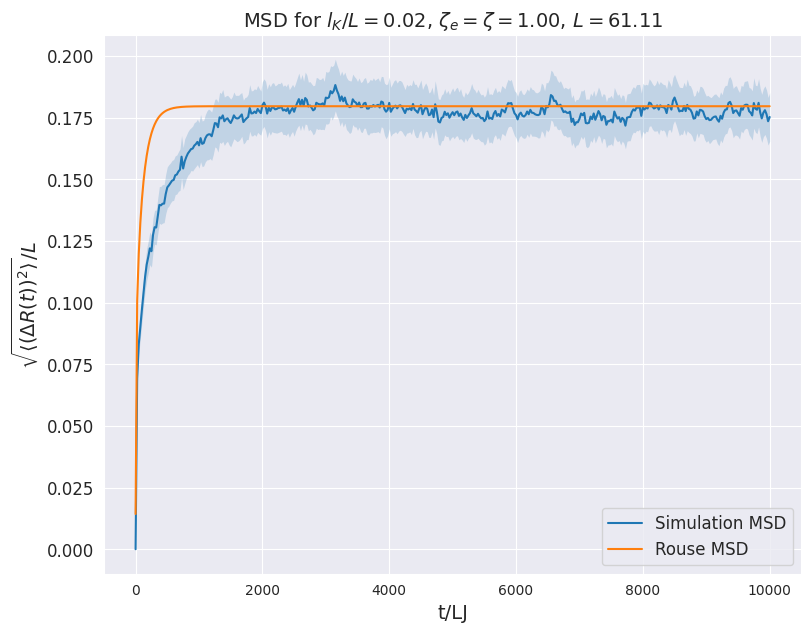
\includegraphics[trim={0.1cm 0.1cm 0.1cm 1cm},clip,height=6.9cm]{./3-exp-fixed-param.png}
        \caption{MSD - compare simulation and Rouse model with $\tau_R$ calculated analytically.}
        \label{fig:full-flex-chain-fixed}
    \end{figure}
\end{frame}


\begin{frame}
    \frametitle{Experiment 1: Fully flexible chain}
    \framesubtitle{$\tau_R$ as free parameter}

    \begin{figure}[h]
        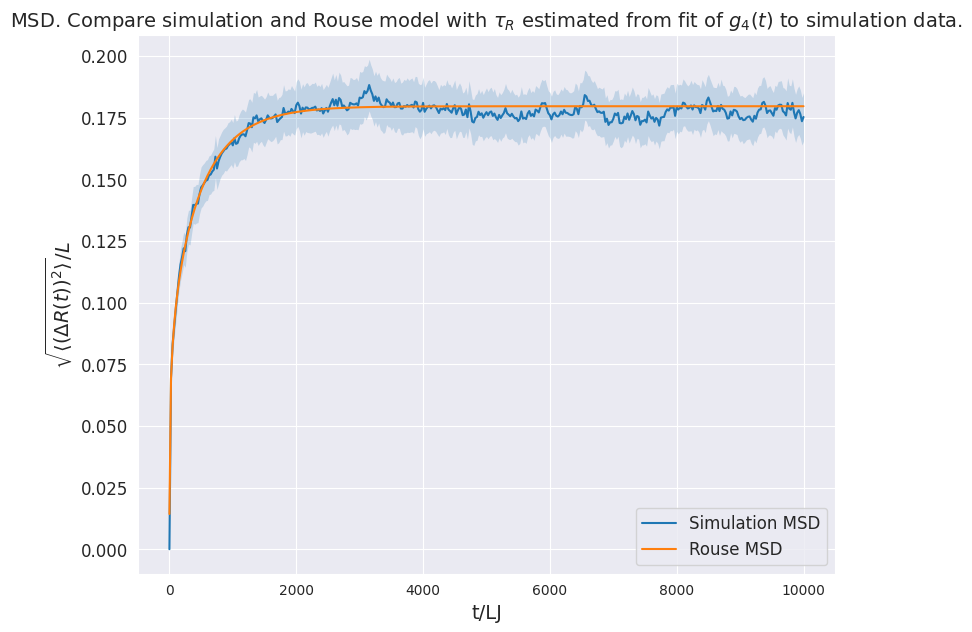
\includegraphics[trim={0.1cm 0.1cm 0.1cm 1cm},clip,height=6.5cm]{./3-exp-free-param.png}
        \caption{MSD - compare simulation and Rouse model 
        with $\tau_R$ estimated from fit of $g_4(t)$ to simulation data.}
        \label{fig:full-flex-chain-free}
    \end{figure}
\end{frame}

\begin{frame}
    \frametitle{Experiment 1: Fully flexible chain}
    \framesubtitle{$\tau_R$ as free parameter}

    \begin{figure}[h]
        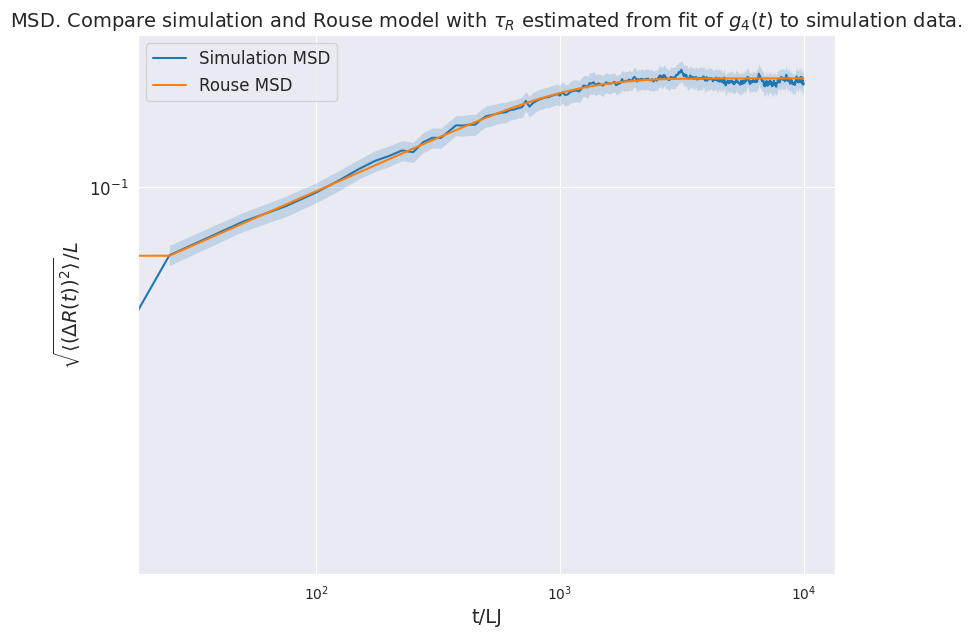
\includegraphics[trim={0.1cm 0.1cm 0.1cm 1cm},clip,height=6.5cm]{./3-exp-free-param-log.png}
        \caption{MSD - compare simulation and Rouse model 
        with $\tau_R$ estimated from fit of $g_4(t)$ to simulation data.}
        \label{fig:full-flex-chain-free-log}
    \end{figure}
\end{frame}


\begin{frame}
    \frametitle{Experiment 1: Fully flexible chain}
    \framesubtitle{$\tau_R$ analytcal/free values}

    Analytical: $\tau_R=130.16$, $\tau_0=0.941$
    \\
    Free parameter: $\tau_R=582.3 \pm 28.6$, $\tau_0=4.21 \pm 0.07$
    \\
    \vspace{1cm}
    Define adjustment factor
    $ \alpha := \frac{\tau_{0, \textrm{empirical}}}{\tau_{0, \textrm{analytical}}} \approx 4.47$
\end{frame}

\begin{frame}
    \frametitle{Experiment 1: Fully flexible chain}
    \framesubtitle{Conclusions / Results}
    \begin{itemize}
        \item Boundary conditions of Rouse model must be adjusted to describe dynamics on 
        short/interim time-scales.
        \item Rouse model with $\tau_R$ as free parameter is introduced to account for boundary
        conditions. Based on $\tau_R$ estimate the adjustment factor for $\tau_0$ is calculated.
        This allows to use the model on chains with different number of segments.

    \end{itemize}
\end{frame}

\section{Experiment 2: Semi-flexible chain, vary persistence length}

\begin{frame}
    \frametitle{Experiment 2: Semi-flexible chain, vary persistence length}
    \framesubtitle{Settings}
    Same potentials used as in \cite[Section 2.1]{svaneborg_2020}, except:
    \begin{itemize}
        \item Only bonded beads interract
    \end{itemize}
\end{frame}

\begin{frame}
    \frametitle{Experiment 2: Semi-flexible chain, vary persistence length}
    \framesubtitle{Used equations}

    Kuhn length \cite{svaneborg_2020}:
    \begin{equation}
        l_K = l_b \frac{2\kappa + e^{-2 \kappa} - 1}{1-e^{-2\kappa}(2 \kappa + 1)}
    \end{equation}
    Number of Kuhn segments:
    \begin{equation} 
        N_K = \frac{L}{l_K}
    \end{equation}
    Rouse time:
    \begin{equation} \label{eq:tau_R_kuhn}
        \tau_R = \frac{1}{3 \pi^2} \frac{\zeta_{K} \mean{R^2}}{k_B T} = \frac{1}{3 \pi^2} \frac{\zeta N_b N_K l_K^2}{k_B T}
    \end{equation}
\end{frame}


\begin{frame}
    \frametitle{Experiment 2: Semi-flexible chain, vary persistence length}
    \framesubtitle{ETE in equilibrium}

    \begin{figure}[h]
        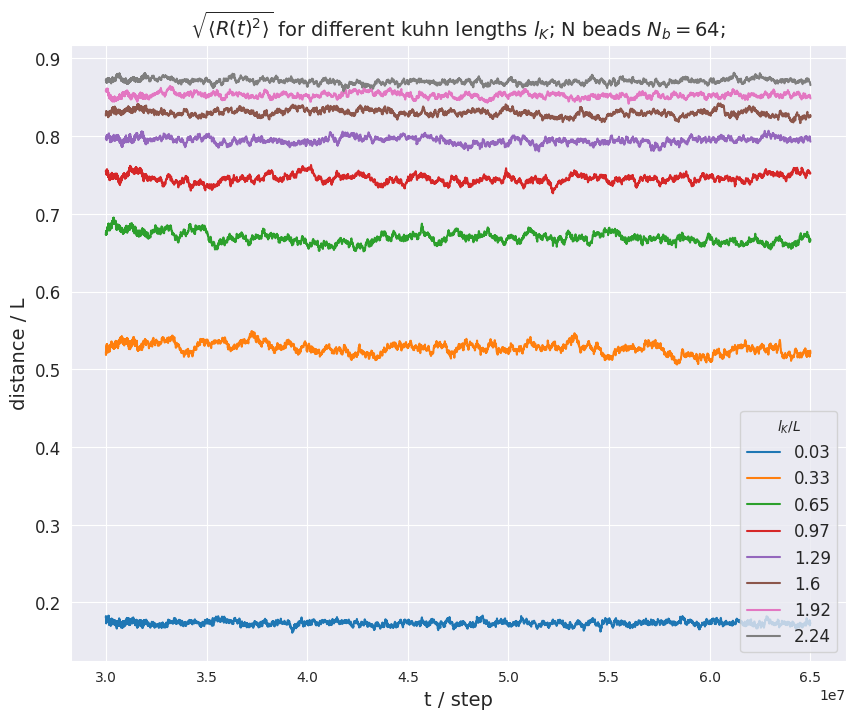
\includegraphics[width=8cm]{./4-exp-R_equi.png}
    \end{figure}
\end{frame}


\begin{frame}
    \frametitle{Experiment 2: Semi-flexible chain, vary persistence length}
    \framesubtitle{ETE vs Kuhn length}

    \begin{figure}[h]
        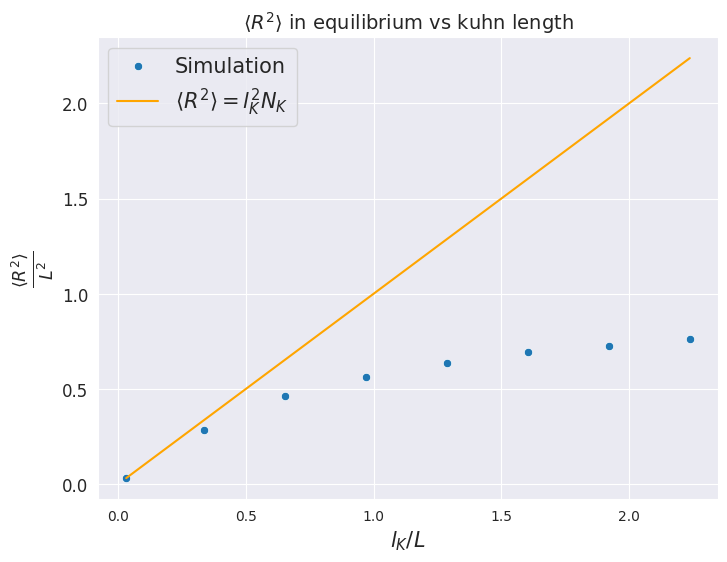
\includegraphics[width=8cm]{./4-exp-R_sim_vs_theor.png}
    \end{figure}
\end{frame}


\begin{frame}
    \frametitle{Experiment 2: Semi-flexible chain, vary persistence length}
    \framesubtitle{MSD: $\mean{[\Delta R(t)]^2}$}

    \begin{figure}[h]
        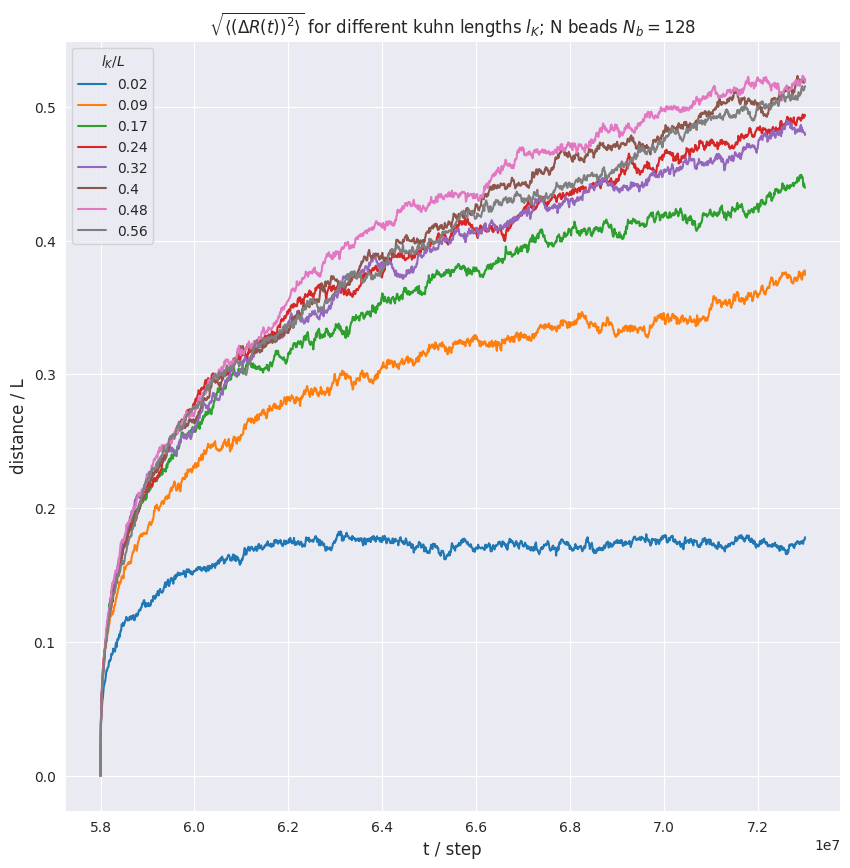
\includegraphics[width=9.5cm]{./4-exp-delta_R-bare.png}
    \end{figure}
\end{frame}

\begin{frame}
    \frametitle{Experiment 2: Semi-flexible chain, vary persistence length}
    \framesubtitle{MSD: $\mean{[\Delta R(t)]^2}$ on log-log scale}

    \begin{figure}[h]
        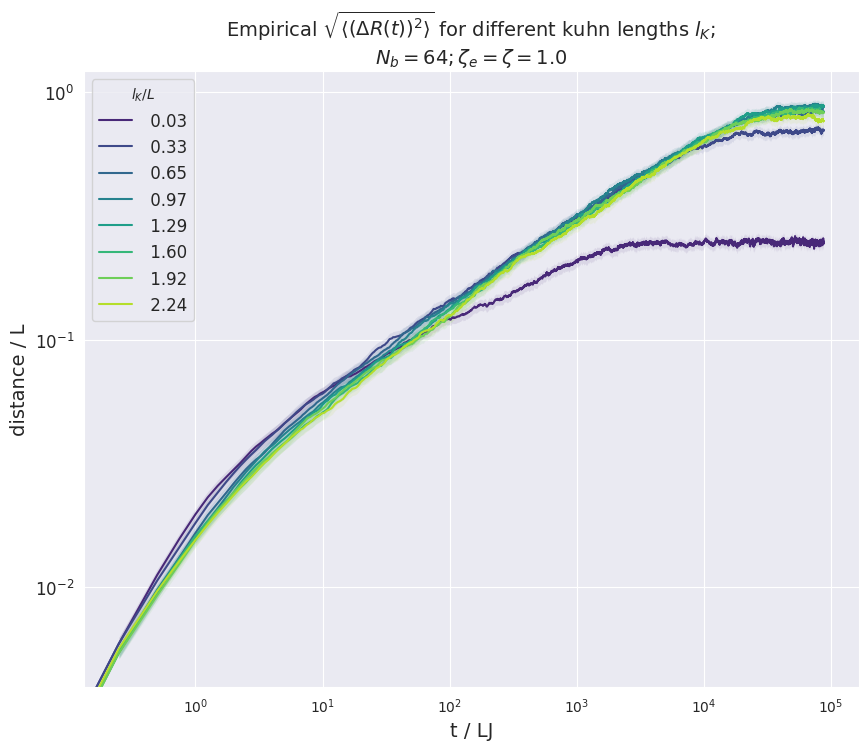
\includegraphics[width=9.5cm]{./4-exp-msd-log.png}
    \end{figure}
\end{frame}

\begin{frame}
    \frametitle{Experiment 2: Semi-flexible chain, vary persistence length}
    \framesubtitle{MSD: $\mean{[\Delta R(t)]^2}$ by dimension}

    \begin{figure}[h]
        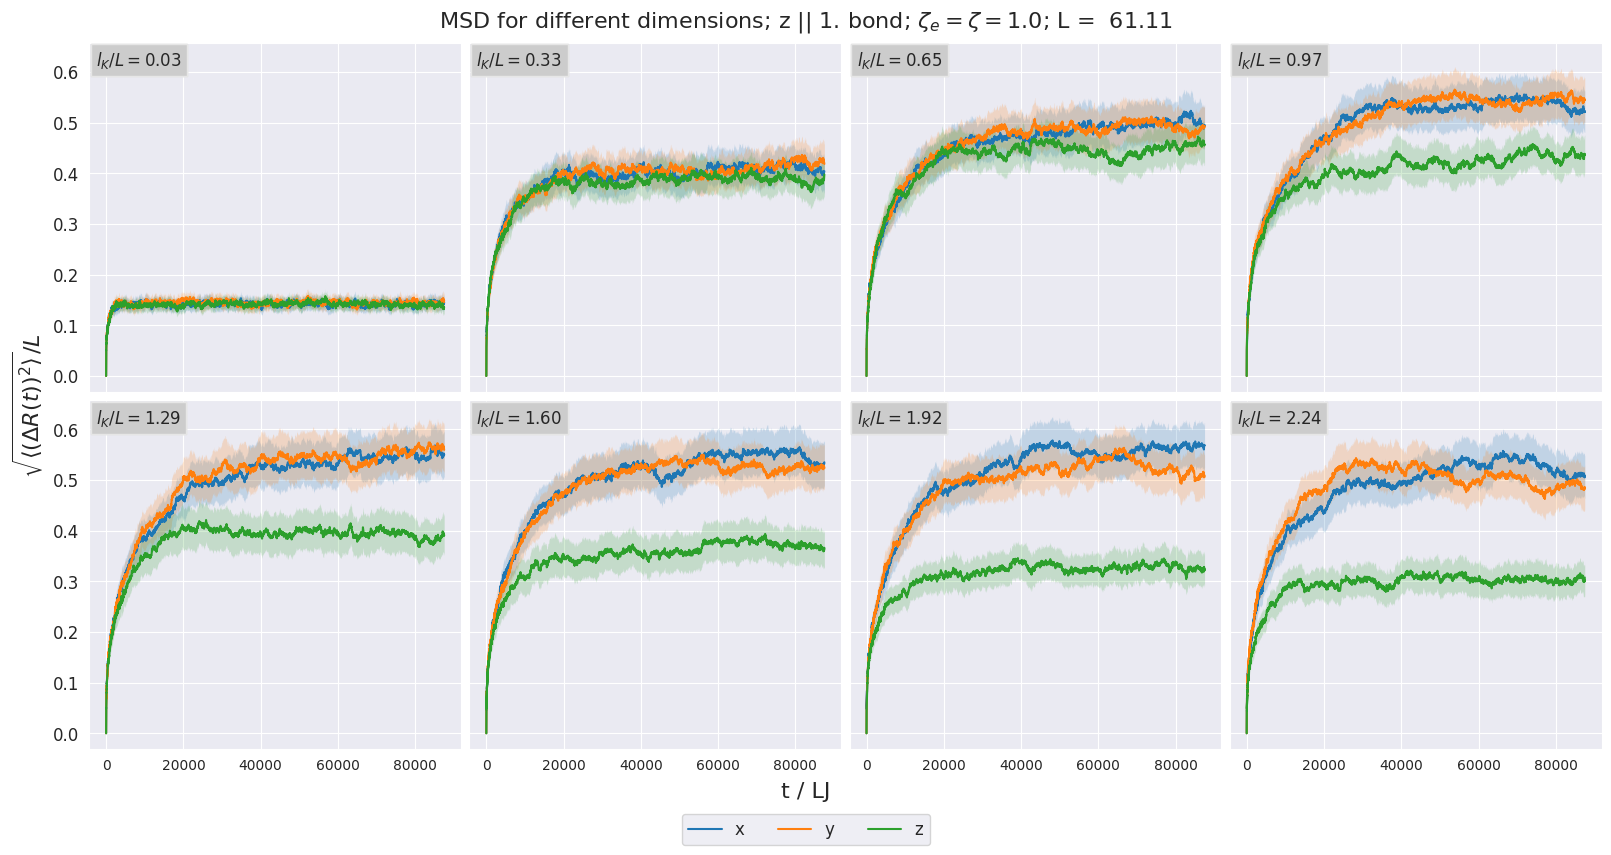
\includegraphics[width=11cm]{./4-exp-msd_by_dim.png}
    \end{figure}
\end{frame}

\begin{frame}
    \frametitle{Experiment 2: Semi-flexible chain, vary persistence length}
    \framesubtitle{MSD: $\mean{[\Delta R(t)]^2}$ by dimension on log scale}

    \begin{figure}[h]
        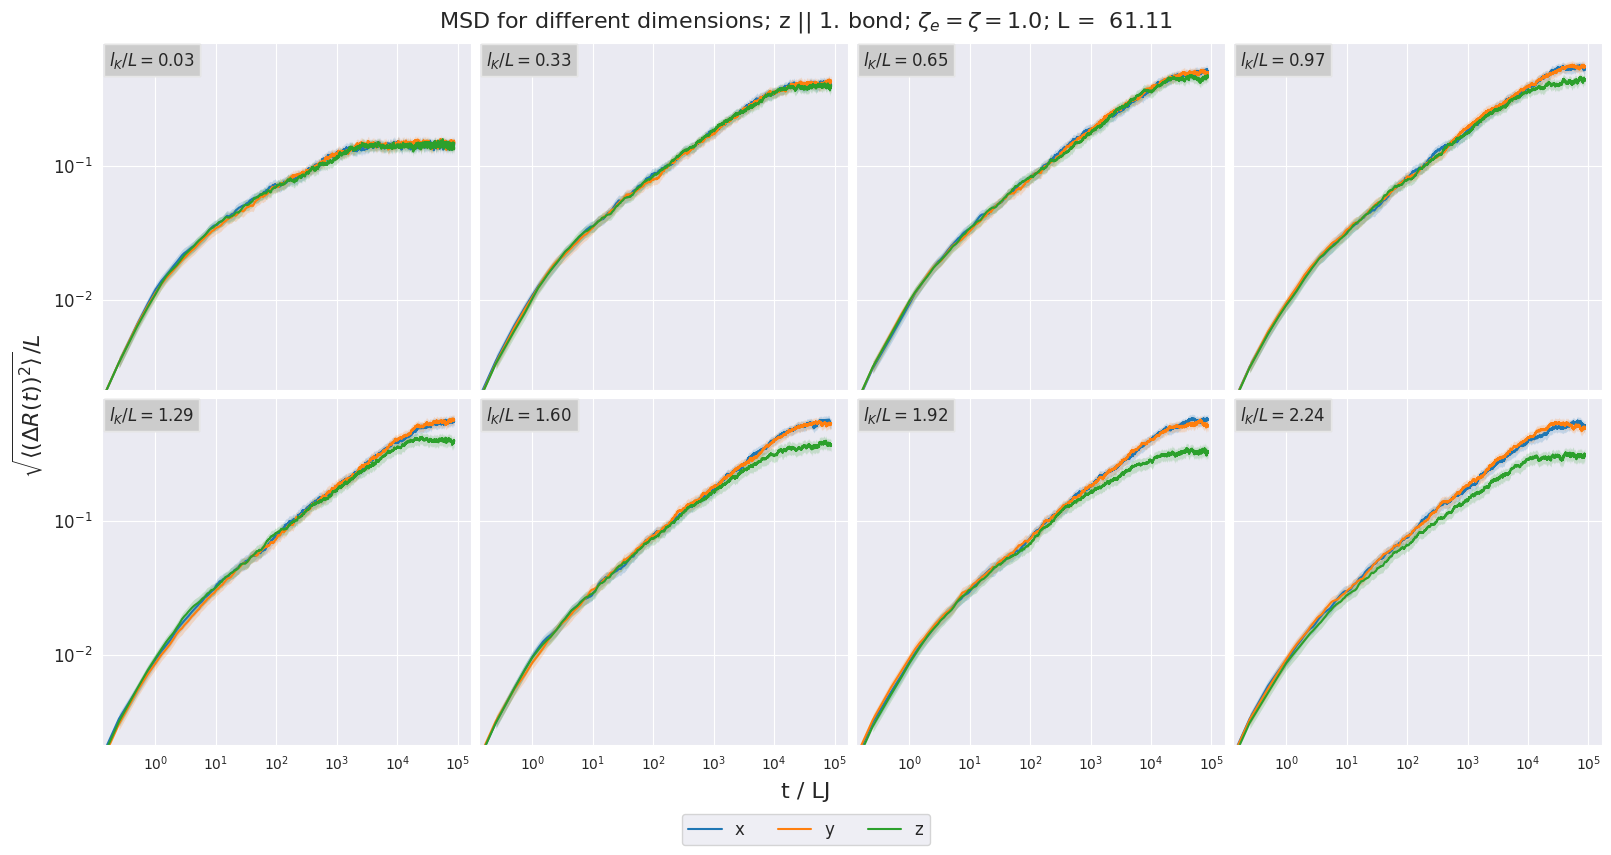
\includegraphics[width=11cm]{./4-exp-msd_by_dim-log.png}
    \end{figure}
\end{frame}

\begin{frame}
    \frametitle{Experiment 2: Semi-flexible chain, vary persistence length}
    \framesubtitle{Conclusions 1}

    \begin{enumerate}
        \item The behavior of MSD for different $l_K$ is roughly the same for $l_K/L \gtrapprox 0.65$
        \item The relaxation time grows non-linearly with rising $l_K$
        \item MSD in z dimension is noticable different for $l_K \gtrapprox 0.97$. 
        \begin{itemize}
            \item The relaxation time in z dimension gets smaller 
            relative to x,y dimensions with increasing $l_K$. Explanation: chain has less freedom along z axis with rising $l_K$. 
            \item MSD is in z is smaller then in x,y on longer time scales. Explanation: same.
        \end{itemize}
    \end{enumerate}
\end{frame}

\begin{frame}
    \frametitle{Experiment 2: Semi-flexible chain, vary persistence length}
    \framesubtitle{$\mean{[\Delta R(t)]^2}$ vs Rouse with $\tau_R$ analytically}

    \begin{figure}[h]
        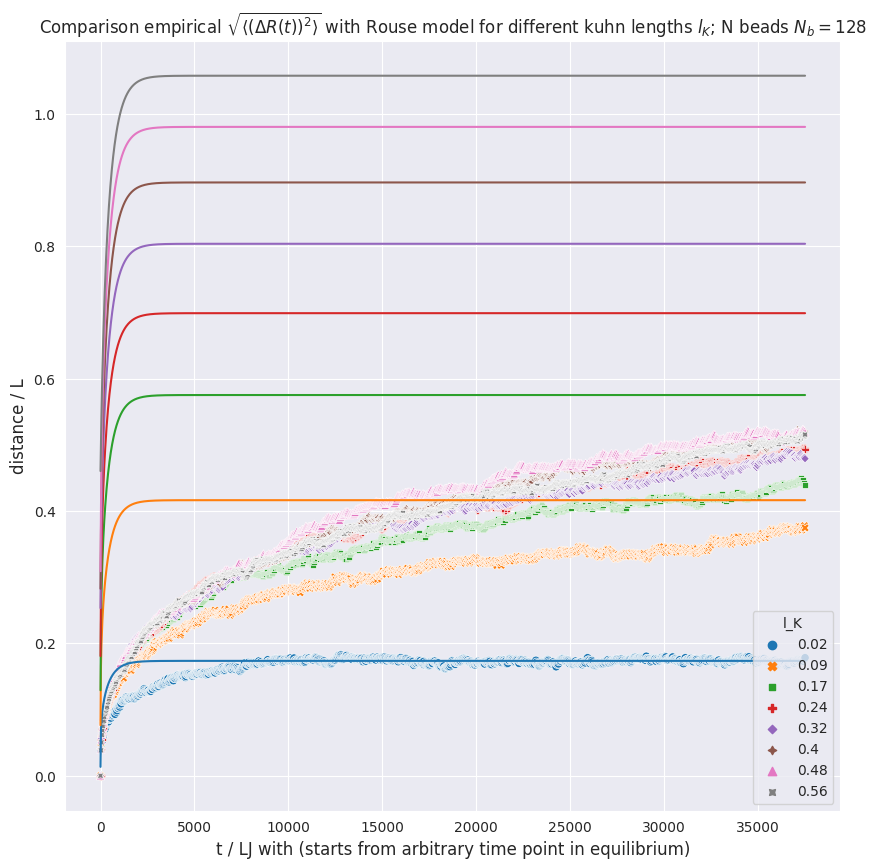
\includegraphics[width=11cm]{./4-exp-delta_R-rouse_anal.png}
    \end{figure}
\end{frame}


\begin{frame}
    \frametitle{Experiment 2: Semi-flexible chain, vary persistence length}
    \framesubtitle{$\mean{[\Delta R(t)]^2}$ vs Rouse with $\tau_R$ as free parameter}

    \begin{figure}[h]
        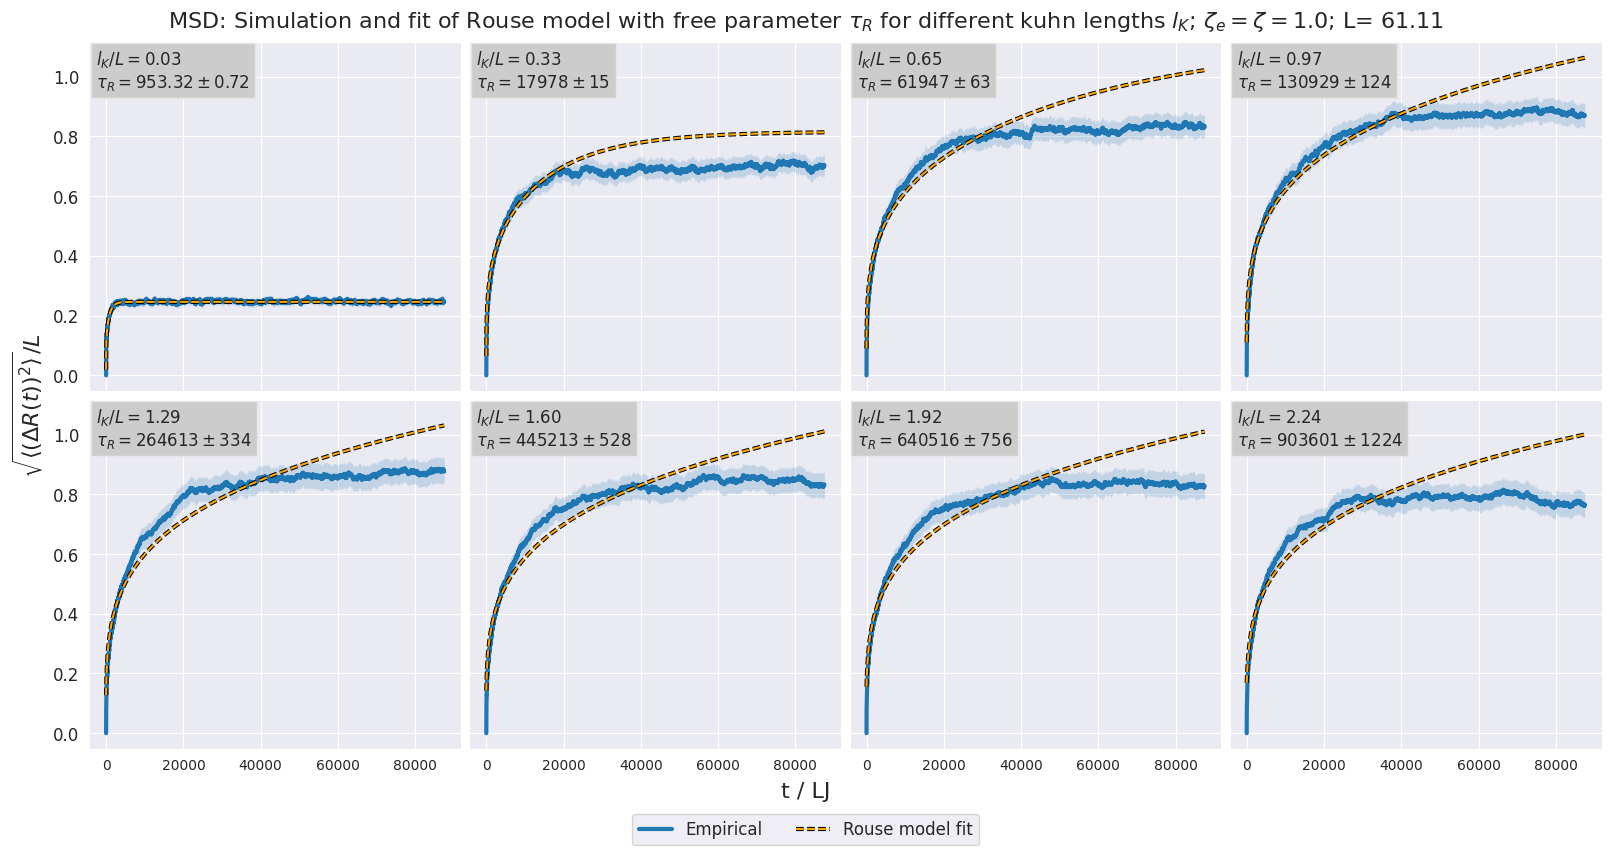
\includegraphics[width=11cm]{./4-exp-delta_R-rouse_fit-tau.png}
    \end{figure}
\end{frame}

\begin{frame}
    \frametitle{Experiment 2: Semi-flexible chain, vary persistence length}
    \framesubtitle{$\mean{[\Delta R(t)]^2}$ vs Adjusted Rouse with $\tau_R$, $a$ as free parameter}
    $$ \mean{[\Delta R(t)]^2} = a \mean{R} [1 - \exp(-\frac{t}{\tau_R})] $$
    \begin{figure}[h]
        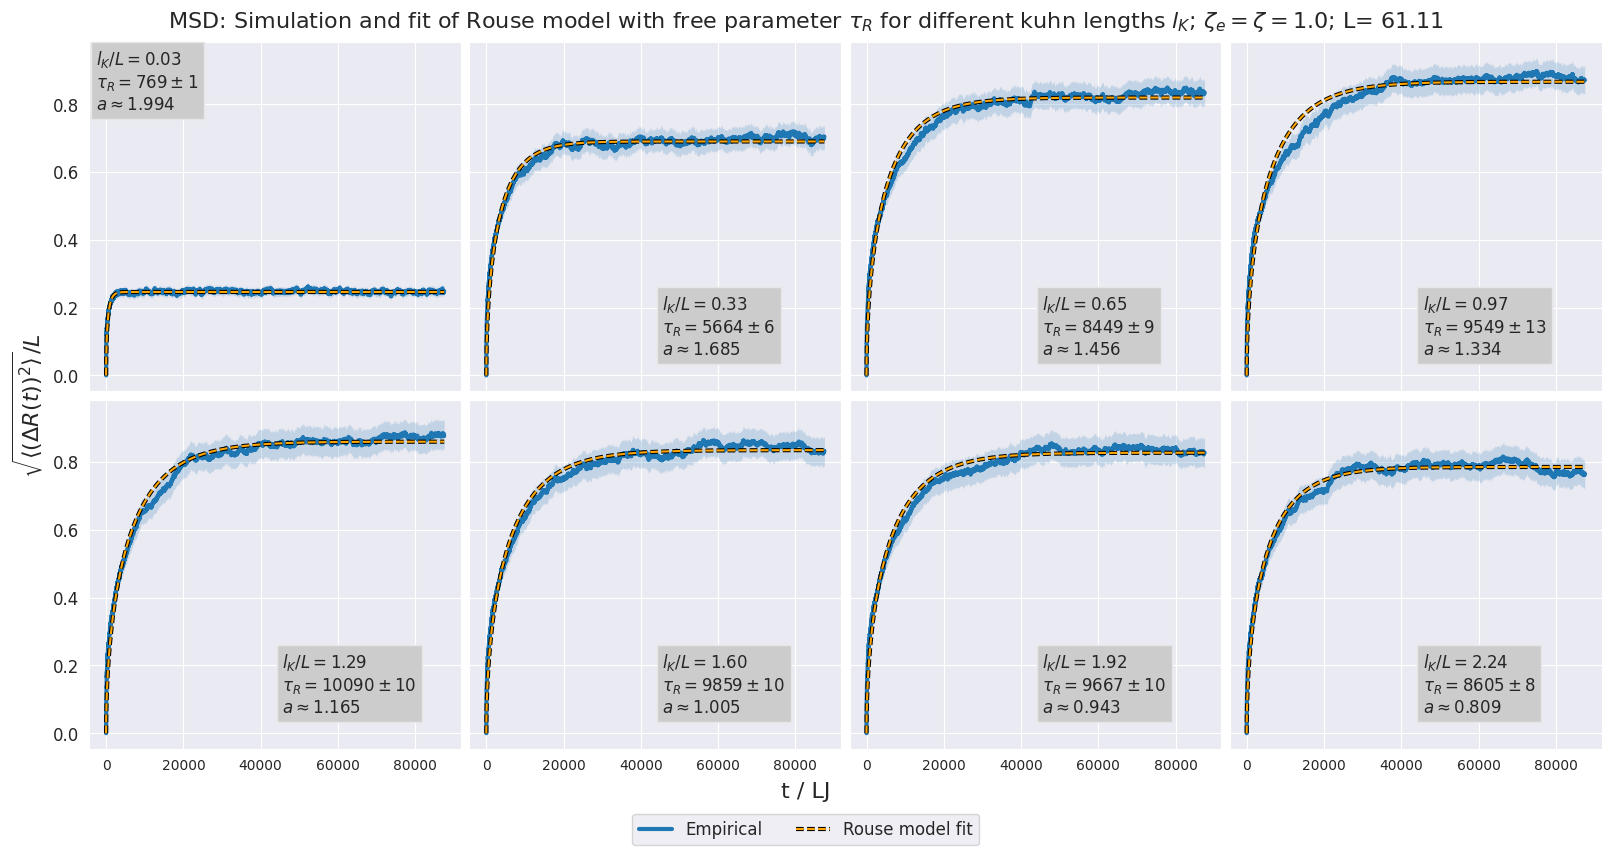
\includegraphics[width=11cm]{./4-exp-delta_R-rouse_fit-tau-a.png}
    \end{figure}
\end{frame}

\begin{frame}
    \frametitle{Experiment 2: Semi-flexible chain, vary persistence length}
    \framesubtitle{$\mean{[\Delta R(t)]^2}$ vs Adjusted Rouse with $\tau_R$, $a$ as free parameter on log scale}
    $$ \mean{[\Delta R(t)]^2} = a \mean{R} [1 - \exp(-\frac{t}{\tau_R})] $$
    \begin{figure}[h]
        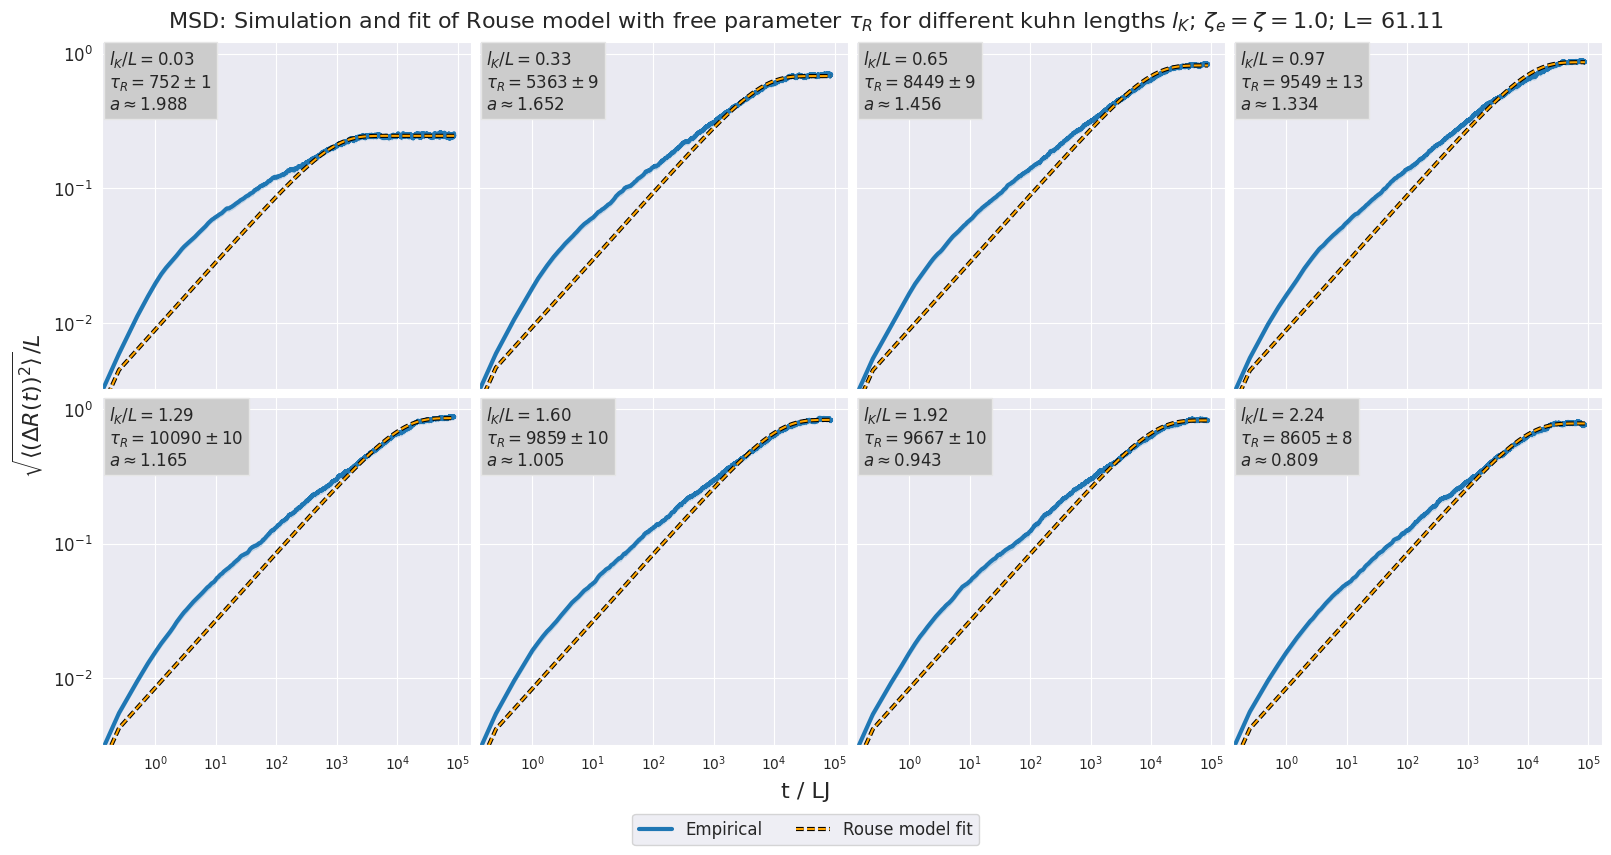
\includegraphics[width=11cm]{./4-exp-delta_R-rouse_fit-tau-a_log.png}
    \end{figure}
\end{frame}

\begin{frame}
    \frametitle{Experiment 2: Semi-flexible chain, vary persistence length}
    \framesubtitle{Conclusions 2}
    \begin{enumerate}
        \item Rouse model is not able to describe semi-flexible chain with $\gtrapprox$ 3 segments
        even with rouse time adjusted for boundary conditions. (Continuum assumption violated.)
        \item Rouse model with free $\tau_R$ doesn't work for small number 
        of kuhn segments.
        \item Introducion of Adjusted Rouse model helps to describe dynamics on 
        interim and large time scales, however it's inaccurate on short time scales.
    \end{enumerate}
\end{frame}

\section{Experiment 3: EEA1/EEA1+Rab5-like chain}

\begin{frame}
    \frametitle{Experiment 3: EEA1/EEA1+Rab5-like chain}
    \framesubtitle{Settings}
    Same potentials used as in \cite[Section 2.1]{svaneborg_2020}, except:
    \begin{itemize}
        \item Only bonded beads interract
    \end{itemize}
    Modelling EEA1 and EEA1+Rab5:
    \begin{itemize}
        \item EEA1: $\kappa = 190.2 \Rightarrow l_K/L=6.02$ 
        \item EEA1+Rab5: $\zeta_e = 10\zeta, 20\zeta$; $m_e=1.5m$
    \end{itemize}
\end{frame}

\begin{frame}
    \frametitle{Experiment 3: EEA1/EEA1+Rab5-like chain}
    \framesubtitle{}
    \begin{figure}[h]
        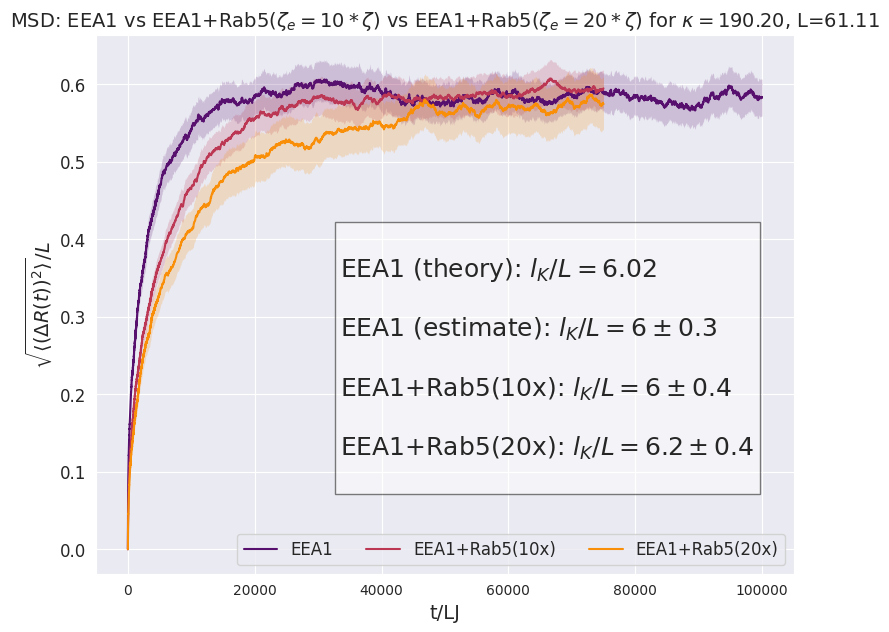
\includegraphics[width=11cm]{./14+15+16-exp-msd.png}
    \end{figure}
\end{frame}

\begin{frame}
    \frametitle{Experiment 3: EEA1/EEA1+Rab5-like chain}
    \framesubtitle{}
    \begin{figure}[h]
        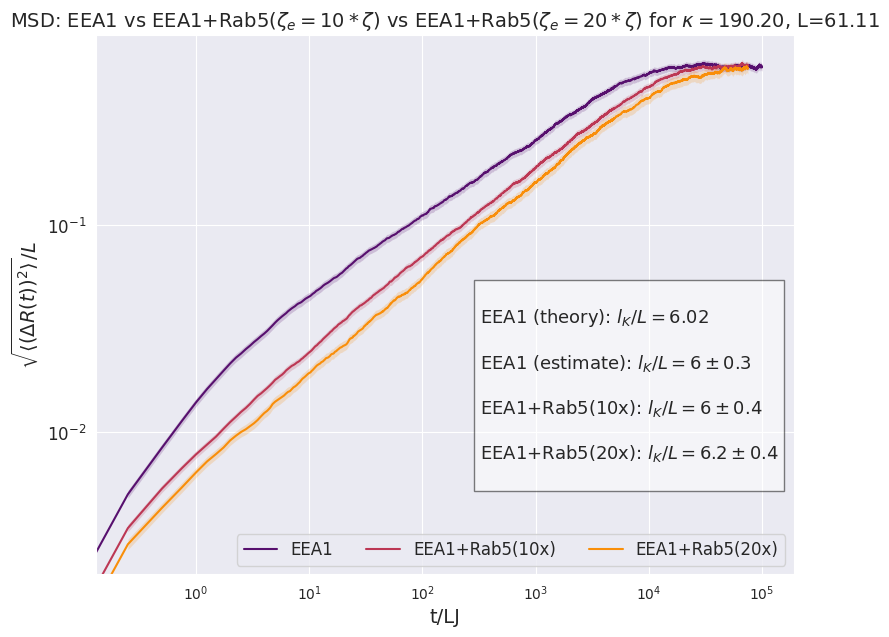
\includegraphics[width=11cm]{./14+15+16-exp-msd-log.png}
    \end{figure}
\end{frame}

\begin{frame}
    \frametitle{Problems and Questions}
    \begin{enumerate}
        \item Eq. (\ref{eq:tau_R_kuhn}): Is the assumption correct? 
        Intuitively: $\zeta_{CM}=\zeta_K N_K=\zeta \frac{N_b}{N_K} N_K=\zeta N_b$, but then
        \cite[Eq. 15]{svaneborg_2020} is not proportional to $N_K^2$.
        \item Empirical $\tau_0$ are with factor $\approx 10^3$ larger then theoretical, why?
    \end{enumerate}
\end{frame}

\section{References}

\setbeamertemplate{bibliography item}{\insertbiblabel}
\begin{frame}
    \frametitle{References}
    \bibliographystyle{apalike}
    \bibliography{refs}
\end{frame}

\end{document}